\chapter{Attributes}
\label{ch:attributes}
This chapter contains the selected \glspl{attribute} for further research. Are the \glspl{attribute} success factors that positively influence the contribution of \acrlong{ea} in achieving \gls{antifragility} in the \gls{ps}? This chapter contains the attributes of \gls{antifragile} and the attributes of \acrlong{ea}. 

After the first selection by using the criteria as definied in \cref{sub:literaturestudy}
\section{Attributes of antifragile}
\label{sec:attributesofantifragile}
\label{sec:attributesantifragile}
\label{sub:attributeseaal}
\textcites{Botjes2020}{Botjes2021} conducted an extensive literature study on \gls{antifragility} and organisation design. \textcites{Botjes2020}{Botjes2021} used the literature study to define \gls{antifragility} and \gls{antifragile} \glspl{attribute} relevant for organisational design. \textcite[Fig.~8]{Botjes2021} created a summary that contains all validated attributes, the \acrlong{eaal}.
\begin{figure}[H]
	\centering
	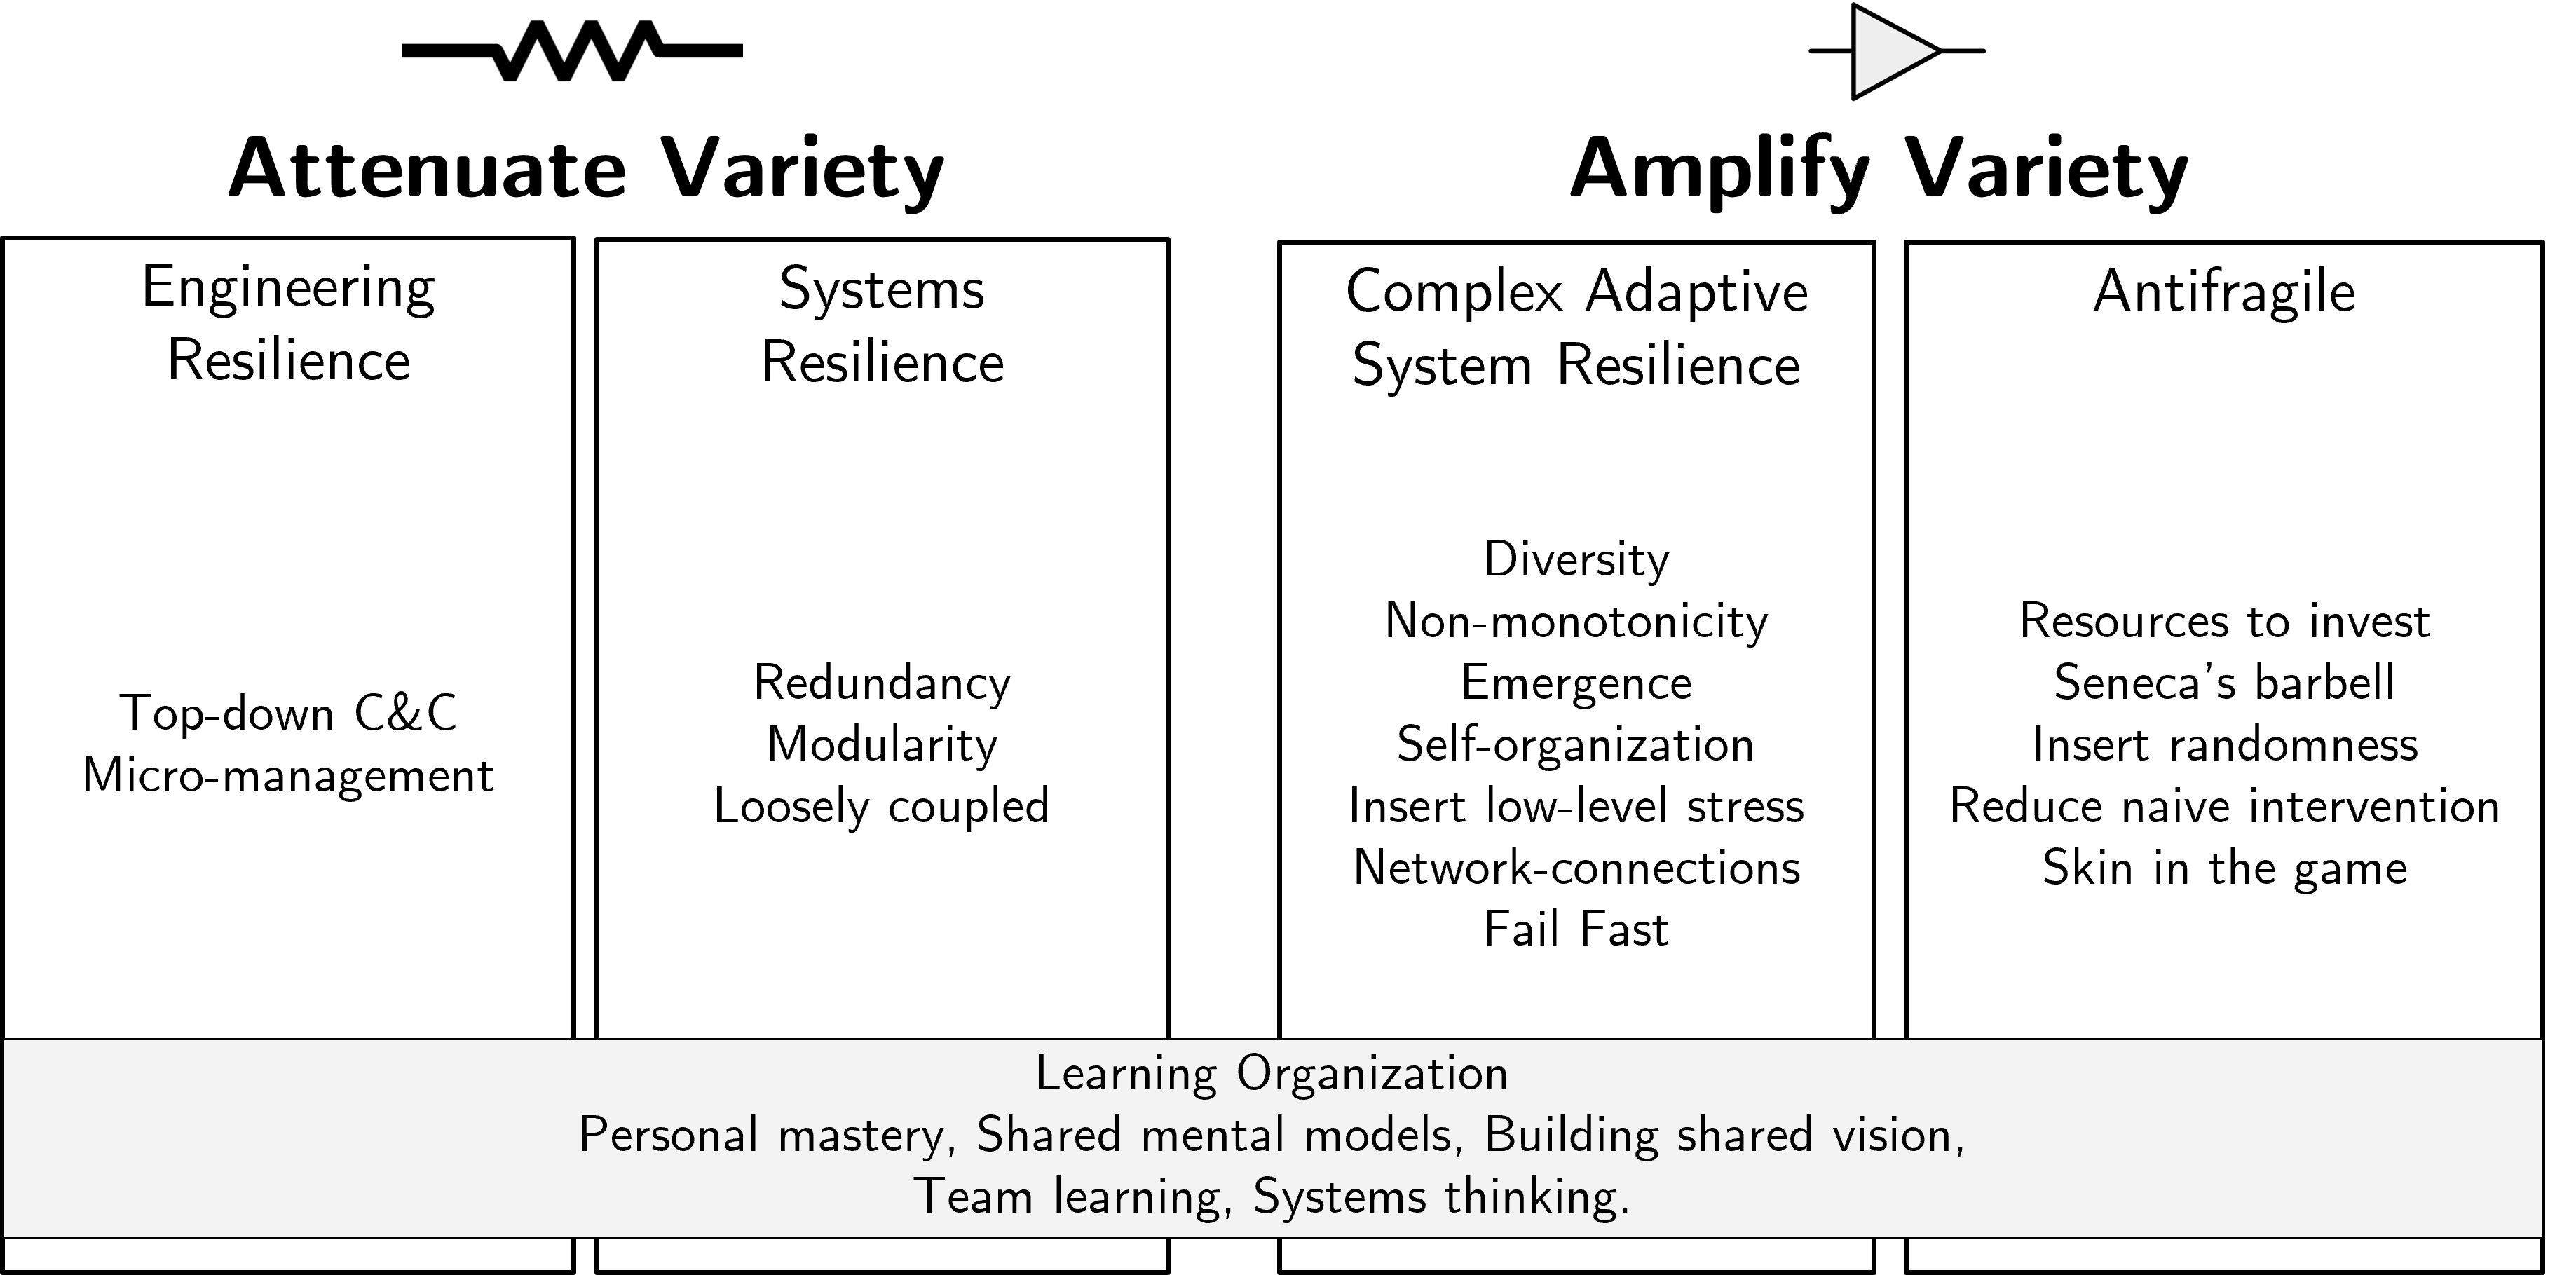
\includegraphics[width=0.8\linewidth]{images/eaalbw}
	\caption[The Extended Antifragile Attribute List \parencite{Botjes2021}]{The Extended Antifragile Attribute List \parencite{Botjes2021}}
	\label{fig:eaalbw}
\end{figure}
According to \textcite[p.~64]{Botjes2020} it is stated by \textcite{Taleb2008} that the following attributes are essential for an \gls{antifragile} system: \Gls{optionality}, \Gls{resourcestoinvest}, \Gls{senecabarbell}, \Gls{insertrandomness}, \Gls{reducenaiveintervention}, and \Gls{skininthegame}. \textcite[p.~64]{Botjes2020} explains that \gls{optionality} is excluded because of the overlap with \gls{diversity}. It is understandable that \textcite[p.~66]{Botjes2020} merges both attributes into one, (\gls{diversity}). They are both much alike. But \textcites{Taleb2012}{Gorgeon2015} both use the term \gls{optionality}. \Gls{optionality} is the availability of options \parencites[p.~176--177]{Taleb2012}[p.~9]{Gorgeon2015}. \Gls{optionality} is an idea advanced by \textcite{Taleb2012}. At the most basic level, \gls{optionality} just means having lots of options. E.g. if you develop a skill with many possible job opportunities, you have more \gls{optionality} than someone who develops a skill that only has one or two job opportunities. For \gls{diversity} \textcite{Botjes2020} used a definition of internally not being a mono-culture and externally having options. E.g. having two different coffee suppliers or having a diverse team. \textcite[Table II]{Botjes2021} refined the definition by adding optionality ''Diversity is the ability to solve a problem in more than one way with different components. Optionality, the availability of options, is a specialisation of diversity. An example is that within a team you want diverse co-workers since other types of people come up with other types of solutions.'' The difference between \gls{optionality} and \gls{diversity} is very subtle. \Gls{optionality} is when you have the right to do something, but you do not have an obligation to do it, where diversity is something that is there or not. It is an option, ''the right but not the obligation'' for the buyer and, of course, ''the obligation but not the right'' for the other party, called the seller \parencite[p.~174]{Taleb2012}. The option is an agent of \gls{antifragility} \parencite[p.~174]{Taleb2012}.\Gls{optionality} allows the buyer to retain the upper bound and be unaffected by adverse outcomes which makes the buyer \gls{antifragile}\footnote{\label{foot:nesslabs}\url{https://nesslabs.com/optionality-fallacy}}. In random, complex environments, convexity, as in \gls{optionality}, is easier to attain than knowledge\cref{foot:nesslabs}. Since this research is about possible success factors and \gls{optionality} is slightly different than \gls{diversity}, \gls{optionality} will be reinstated for further research. With \cref{fig:eaalbwincludingoptionality} the attribute \gls{optionality} is reinstated into the \acrlong{eaal} \parencite[Fig.~8]{Botjes2021} for further research.
\begin{figure}[H]
	\centering
	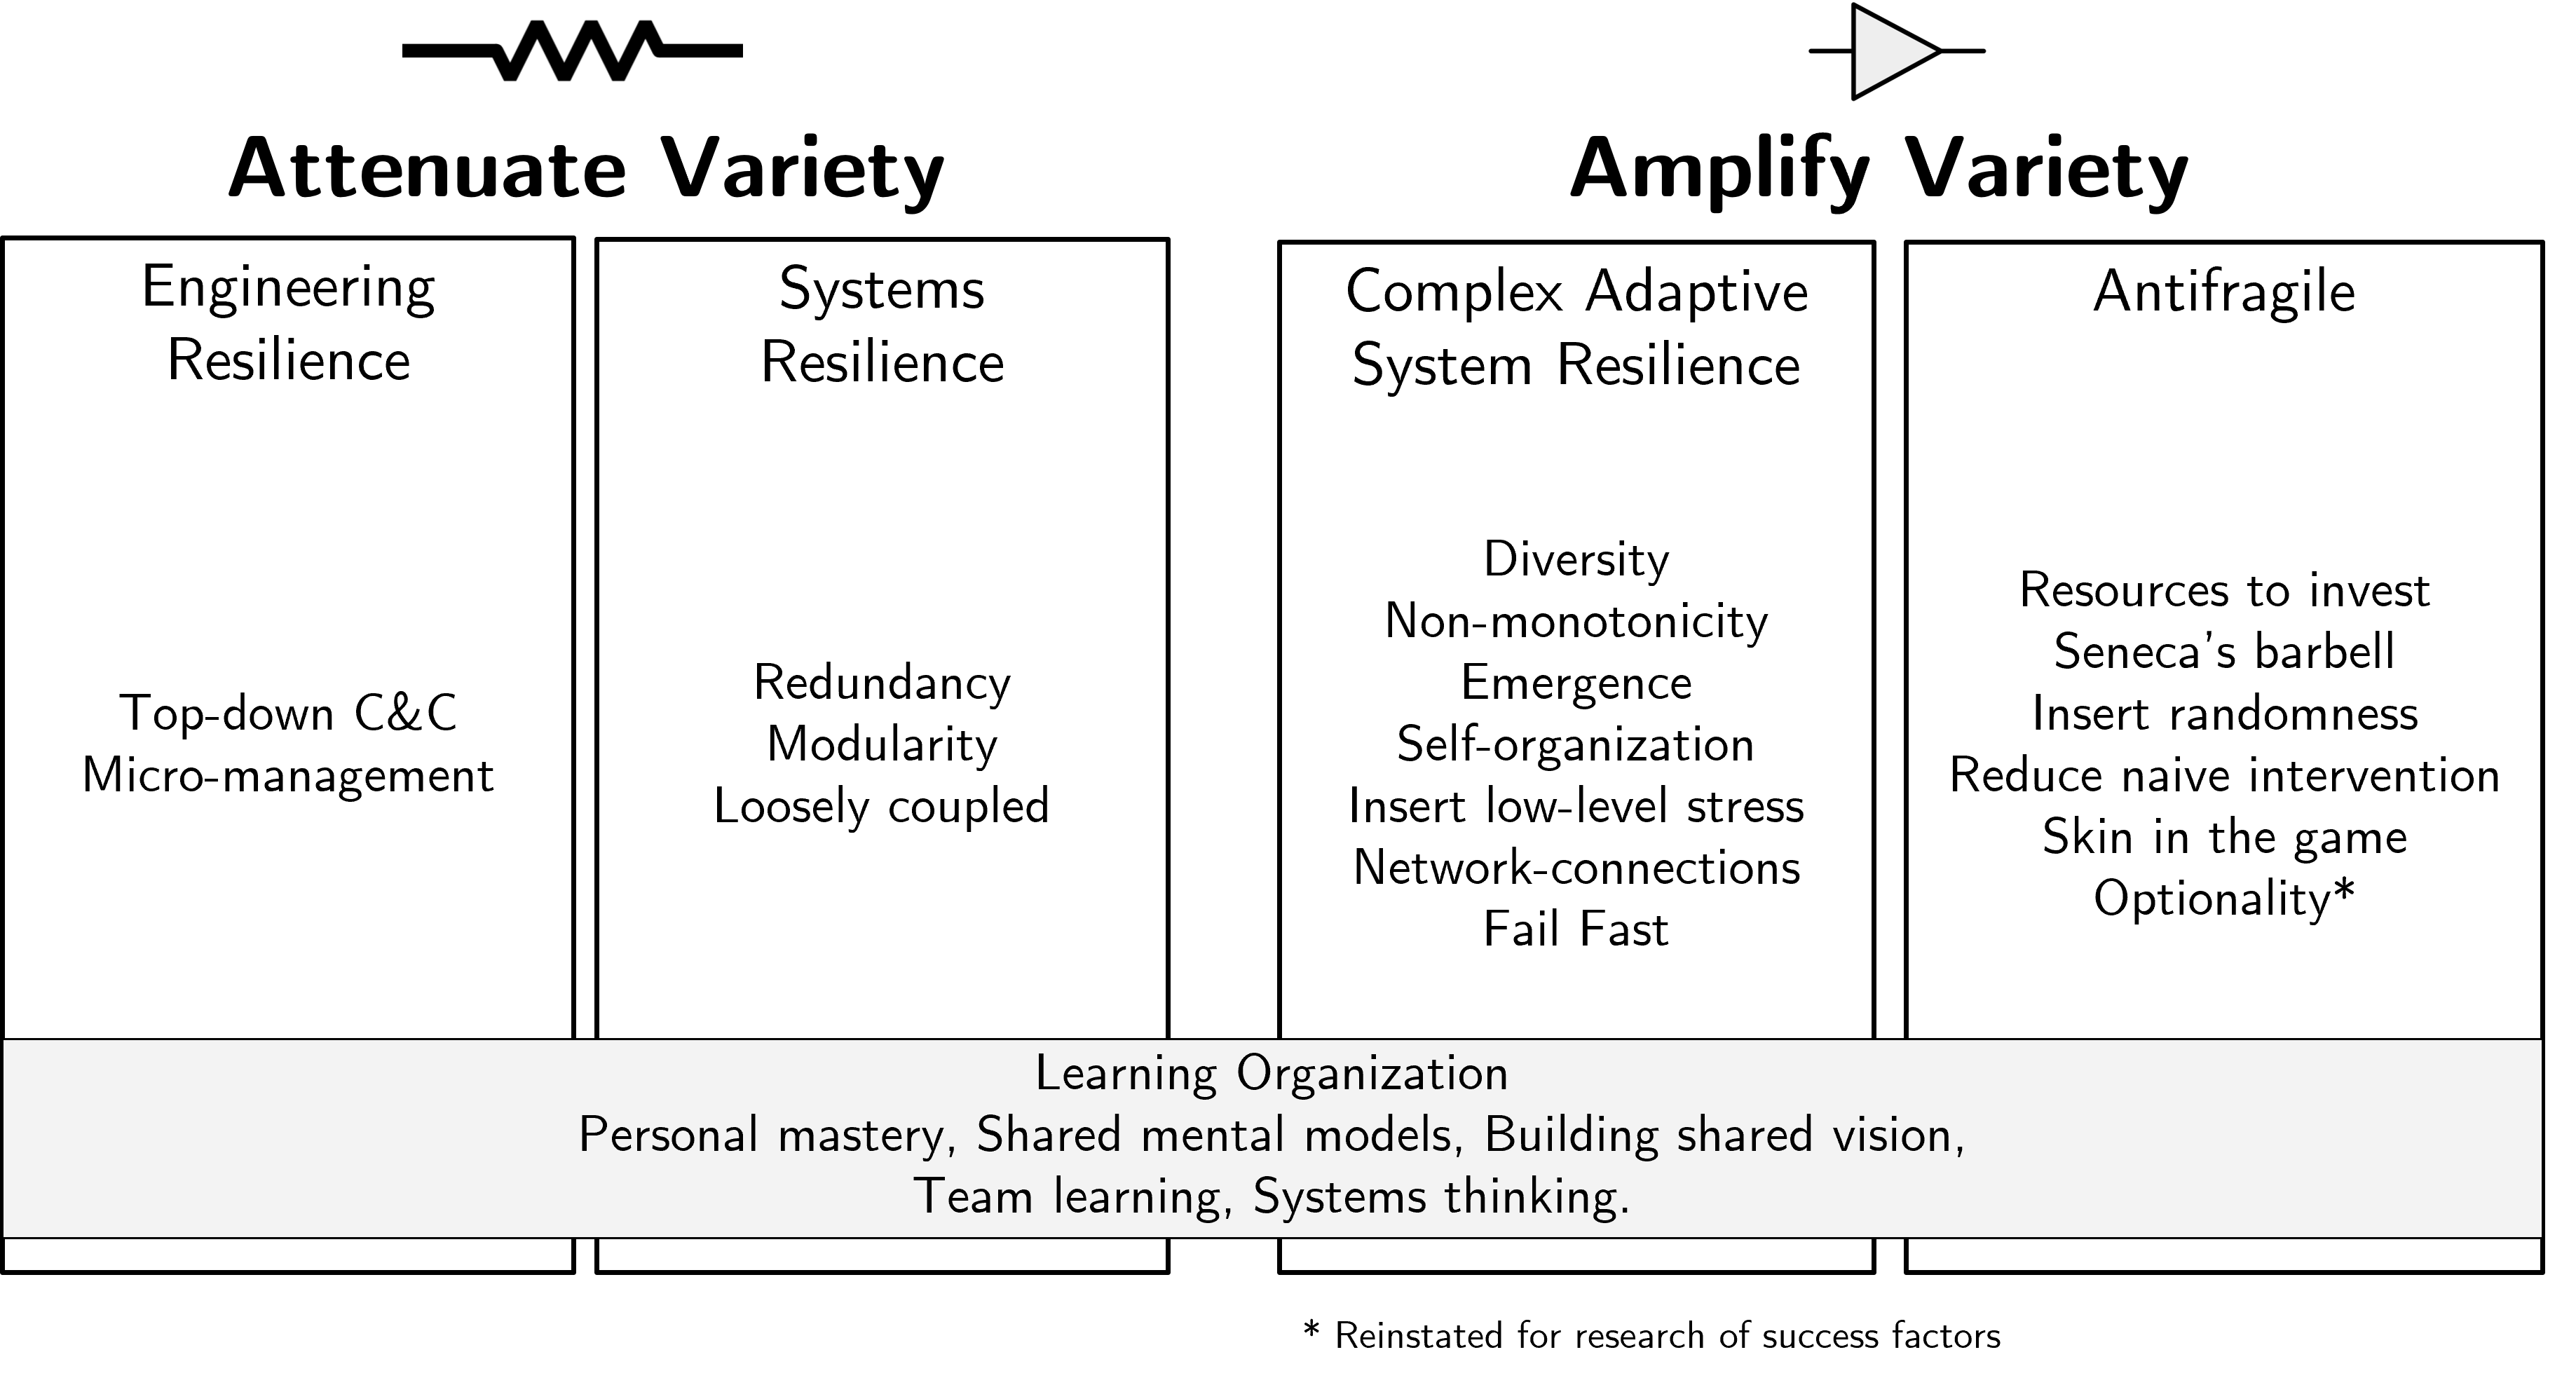
\includegraphics[width=0.8\linewidth]{images/eaalbwincludingoptionality}
	\caption[The Extended Antifragile Attribute List \parencite{Botjes2021} with optionality reinstated]{The Extended Antifragile Attribute List \parencite{Botjes2021} with optionality reinstated}
	\label{fig:eaalbwincludingoptionality}
\end{figure}
\textcite{Botjes2021} used three categories to sort attributes based on behaviour. The first two categories are defined by \textcite[p.~4]{Botjes2021} as a type of variety, see \cref{sub:attenuatevsaplify}, \textit{\gls{attenuatevariety}} and \textit{\gls{amplifyvariety}}. The third category is the \textit{learning organisation} \parencite[p.~4]{Botjes2021}. For this research the most important categories are \textit{\gls{amplifyvariety}} and the \textit{learning organisation}. \Gls{attenuatevariety} leans more towards \gls{robust} and \gls{resilient} and less towards \gls{antifragile}. We use the same categories to sort the \gls{antifragile} attributes.
\subsection{Antifragile attributes}
\label{sub:antifragileattributes}
The \gls{antifragile} \glspl{attribute} that are selected for use for this research are the \gls{antifragile} \glspl{attribute} of the \acrlong{eaal} of \textcite[p.~7]{Botjes2021}. These attributes define our lens on \gls{antifragility} in the \gls{ps}.
\begin{table}[H]
	\begin{center}
			\begin{tabular}{@{}ll@{}}
				\multicolumn{2}{c}{\textbf{\Gls{attenuatevariety} \glspl{attribute}}} \\%
				\toprule %
				\textbf{\Gls{attribute}} & \textbf{Sources} \\%
				\midrule %
				\Gls{topdowncc} & \parencite{Botjes2021} \\%
				\Gls{micromanagement} & \parencite{Botjes2021} \\%
				\Gls{redundancy} & \parencite{Botjes2021} \\%
				\Gls{modularity} & \parencite{Botjes2021} \\%
				\Gls{looselycoupled} & \parencite{Botjes2021} \\%
			\bottomrule%
			\end{tabular}
			\caption[\Gls{attenuatevariety} \glspl{attribute} of \gls{antifragile}]{\Gls{attenuatevariety} \glspl{attribute} of \gls{antifragile}}
			\label{tab:attenuatingattributes}
\end{center}
\end{table}				
\begin{table}[H]
	\begin{center}
		\begin{tabular}{@{}ll@{}}
			\multicolumn{2}{c}{\textbf{\Gls{amplifyvariety} \glspl{attribute}}} \\%
			\toprule %
			\textbf{\Gls{attribute}} & \textbf{Sources} \\%
			\midrule%
			\Gls{diversity} & \parencite{Botjes2021} \\%
			\Gls{nonmonotonicity} & \parencite{Botjes2021} \\%
			\Gls{emergence} & \parencite{Botjes2021} \\%
			\Gls{selforganisation} & \parencite{Botjes2021} \\%
			\Gls{insertlowlevelstress} & \parencite{Botjes2021} \\%
			\Gls{networkconnections} & \parencite{Botjes2021} \\%
			\Gls{failfast} & \parencite{Botjes2021} \\%
			\Gls{resourcestoinvest} & \parencites{Taleb2012}{Botjes2021} \\%
			\Gls{senecabarbell} &  \parencites{Taleb2012}{Botjes2021} \\%
			\Gls{insertrandomness} & \parencites{Taleb2012}{Botjes2021} \\%		
			\Gls{reducenaiveintervention} & \parencites{Taleb2012}{Botjes2021} \\%
			\Gls{skininthegame} & \parencites{Taleb2012}{Botjes2021} \\%
			\Gls{optionality} & \parencites{Taleb2012}{Gorgeon2015} \\%
			\bottomrule%
		\end{tabular}
		\caption[Amplify variety attributes of \gls{antifragile}]{Amplify variety attributes of \gls{antifragile}}
		\label{tab:amplifyingattributes}
	\end{center}
\end{table}			
\begin{table}[H]
	\begin{center}
		\begin{tabular}{@{}ll@{}}
			\multicolumn{2}{c}{\textbf{Learning organisation \glspl{attribute}}} \\%
			\toprule %
			\textbf{\Gls{attribute}} & \textbf{Sources} \\%
			\midrule %
			\Gls{personalmastery} & \parencite{Botjes2021} \\%
			\Gls{sharedmentalmodels} & \parencite{Botjes2021} \\%
			\Gls{buildingsharedvision} & \parencite{Botjes2021} \\%
			\Gls{teamlearning} & \parencite{Botjes2021} \\%
			\Gls{systemsthinking} & \parencite{Botjes2021} \\%
			\bottomrule%
		\end{tabular}
		\caption[Learning organisation \glspl{attribute} of \gls{antifragile}]{Learning organisation \glspl{attribute} of \gls{antifragile}}
		\label{tab:learningorganisationattributes}
	\end{center}
\end{table}	
\section{Attributes of Enterprise Architecture}
\label{sec:attributesonea}

\begin{table}[H]%
	\begin{center}%
		\begin{tabular}{@{}ll@{}}%
			\multicolumn{2}{c}{\textbf{\gls{enterpriseitarchitecting} \glspl{enterpriseitarchitecting}}} \\%
			\toprule %
			\textbf{Attribute} & \textbf{Sources} \\%
			\midrule%
			Enable Business Strategy & \parencite{Lapalme2012} \\%
			Support IT planning and cost reduction & \parencite{Lapalme2012} \\%
			Apply a reductionist (mechanistic) stance & \parencite{Lapalme2012} \\%
			Design organisational dimensions independently & \parencite{Lapalme2012} \\%
			\bottomrule%
		\end{tabular}%
		\caption[\Gls{enterpriseitarchitecting} \glspl{attribute}]{\Gls{enterpriseitarchitecting} \glspl{attribute}}%
		\label{tab:attributesofenterpriseitarchitecting}%
	\end{center}%
\end{table}%

\begin{table}[H]%
	\begin{center}%
		\begin{tabular}{@{}ll@{}}%
			\multicolumn{2}{c}{\textbf{\Gls{enterpriseintegrating} \glspl{attribute}}} \\%
			\toprule %
			\textbf{Attribute} & \textbf{Sources} \\%
			\midrule %
			Enable Business Strategy \& Objectives & \parencite{Lapalme2012} \\%
			Apply Systems Thinking & \parencite{Lapalme2012} \\%
			\Gls{intraorganisationalcoherency} & \parencite{Lapalme2012} \\%
			\Gls{holisticsystemicstance} & \parencite{Lapalme2012} \\%
			Managed the Environment & \parencite{Lapalme2012} \\%
			\bottomrule%
		\end{tabular}%
		\caption[\Gls{enterpriseintegrating} \glspl{attribute}]{\Gls{enterpriseintegrating} \glspl{attribute}}%
		\label{tab:attributesofenterpriseintegrating}%
	\end{center}%
\end{table}%

\begin{table}[H]
	\begin{center}
		\begin{tabular}{@{}ll@{}}
				\multicolumn{2}{c}{\textbf{\Gls{enterpriseecologicaladaptation} \glspl{attribute}}} \\%
				\toprule %
				\textbf{Attribute} & \textbf{Sources} \\%
				\midrule%
				\Gls{systeminenvironment} & \parencite{Lapalme2012} \\%
				\Gls{holisticsystemicstance} & \parencite{Lapalme2012} \\%
				\Gls{intraorganisationalcoherency} & \parencite{Lapalme2012} \\%
				\Gls{organisationallearning} & \parencite{Lapalme2012} \\%
				\Gls{environmentallearning} & \parencite{Lapalme2012} \\%
				\Gls{systeminenvironmentcoevolutionlearning} & \parencite{Lapalme2012} \\%
				\bottomrule%
			\end{tabular}
		\caption[\Gls{enterpriseecologicaladaptation} \glspl{attribute}]{\Gls{enterpriseecologicaladaptation} \glspl{attribute}}
		\label{tab:attributesofeea}
	\end{center}
\end{table}
